%!TeX root = Chapter_SignalAnalysisAndCompMeth
\documentclass[../../CompleteThesis2/Complete_2ndDraft]{subfiles}
%\graphicspath{{../../Figures/}}
\begin{document}
The presented data obtained through various experimental measurements (ECM, DEP, isotopic analysis) are easily compared with a time series, as they typically show some quantity measured all along the depth of an ice core. This depth is often, at short intervals, treated as a regular linear time series thus making it possible to use some of the known signal analysis methods. Of course, when considering the entirety of an ice core, the linearity disappears as thinning and compression makes the depth series non linear. But when considering short lengths of core it is possible to estimate a linearity, assuming conformity in this specific layer. 



\section[Spectral Transforms]{Spectral Analysis of Time Series}
\label{Sec:SignalAnalysis_SpectralAnalysis}

%\subsection[Spectral Analysis][Spectral Analysis]{Spectral Analysis}
%\label{Subsec:SignalAnalysis_BackDiffusion_SpectralAnalysis}
\subsection[PSD][PSD]{Power Spectral Densities}
\label{Subsec:SignalAnalysis_BackDiffusion_SpectralAnalysis_PSD}
A very useful tool for analyzing signals exhibiting oscillatory effects is analysis of the signals power spectrum. Instead of considering the signal in time, it is transformed to the spectral domain, where it is possible to obtain an estimate of both the signal and the underlying noise. This is crucial for enhancing the signal and filtering away noise. But to be able to examine these effects, first the data must be transformed. A range of different methods may be used to compute the frequency transform of the depth series, here I present the three I have been working with. Since the data are discrete and experimental, I will be presenting the discrete and applicable mathematical models.\\
When considering a signal, it may be of interest to investigate how the energy of said signal is distributed with frequency. The total power is defined as:
\begin{equation}
	\text{Total Power} = \int_{-\infty}^{\infty} |X(\tau)|^2 \, d\tau.
	\label{Eq:SignalEnergy}
\end{equation}
Using Parseval's theorem (REFERENCE) (assuming that the signal has a finite total energy), the power of the signal can alternatively be written as

\begin{equation}
	\int_{-\infty}^{\infty} |X(\tau)|^2 \, d\tau = \int_{-\infty}^{\infty} |\tilde{X}(\tau)|^2\, df
	\label{Eq:ParsevalsTheorem}
\end{equation}
where $\tilde{X}(f)$ is the spectral (Fourier) transform of the signal, from time to frequency domain, defined as:
\begin{equation}
	\tilde{X}(f) = \int_{-\infty}^{\infty} X(\tau) e^{2\pi i f \tau} \, d\tau
	\label{Eq:FourierTransform}
\end{equation}
and the inverse spectral (Fourier) transform, from frequency to time domain, defined as:
\begin{equation}
	X(t) = \int_{-\infty}^{\infty} \tilde{X}(f) e^{-2\pi i f \tau}\, df.
	\label{Eq:InverseFourierTransform}
\end{equation}
Both $X(t)$ and $\tilde{X}(f)$ represent the same function, just in different variable domains. Often, the angular frequency $\omega$ is used instead, with the relation between $\omega$ and $f$ being $\omega \equiv 2\pi f $, giving the Fourier and inverse Fourier transforms as:

\begin{equation}
	\begin{aligned}
		\tilde{X}(\omega) &= \int_{-\infty}^{\infty} X(t) e^{i\omega\tau}\, d\tau \\
		X(\tau) &= \int_{-\infty}^{\infty} \tilde{X}(\omega) e^{-i\omega\tau}\, d\omega
		\label{Eq:FourierTransformAngular}
	\end{aligned} 
\end{equation}

From Equation \ref{Eq:ParsevalsTheorem} we can interpret the integrand on the right hand side $|\tilde{X}(f)|^2$ as a density function, describing the energy per unit frequency. This is a property which is able to reveal much information about the considered signal, and it is useful to define this as the (one-sided) Power Spectral Density: 
\begin{equation}
	P_X(f) \equiv |\tilde{X}(f)|^2 + |\tilde{X}(-f)|^2 \qquad 0 \leq f < \infty
\end{equation}
This entity ensures that the total power is found just by integrating over $P_X(f)$ from 0 to $\infty$. When the function is purely real, the PSD reduces to $P_X(f) = 2|\tilde{X}(f)|^2$.\\
In the above the transform used to define the PSD was presented as the Fourier transform. When working with discrete data, as is very common when analyzing real world data, there are a number of different ways of estimating the PSD. In the following a number of different transforms will be presented briefly, all used in this thesis.
\newline
\todo{SIGNAL-BACKDIFF: RETHINK THIS PART. DO NOT USE TIME ON ALL THE CALCULATIONS. WRITE THE GENERAL IDEAS OF THE METHODS AND STATE HOW TO CALCULATE/COMPUTE. SMALL CODE SNIP TO GIVE GENERAL IDEA.}



\subsubsection[Spectral Transforms][Spectral Transforms]{Spectral Transforms}
\label{Subsubsec:SignalAnalysis_BackDiffusion_SpectralAnalysis_SpectralTransforms}

\begin{itemize}
	\item DFT/FFT
	\item NUDFT
	\item DCT
	\item NDCT
	%\item (MEM)
\end{itemize}


%\subsection[Back Diffusion]{Back Diffusion Through Spectral Analysis}
%\label{Subsubsec:SignalAnalysis_SpectralAnalysis_BD}


\section[Back Diffusion][Back Diffusion]{Back Diffusion Through Spectral Analysis}
\label{Sec:SignalAnalysis_BackDiffusion}
Due to diffusion in firn and ice, some of the water isotopic signal is lost. Some of this signal can be restored by investigating the diffusion process, and through filtering and deconvolution techniques(REFERENCES).
For the data of this thesis a spectral method, determining the effect of mixing and diffusion as a spectral filter(REFERENCES) is used as a restoration technique. 
	
	
	


\begin{figure}[h]
	\centering
	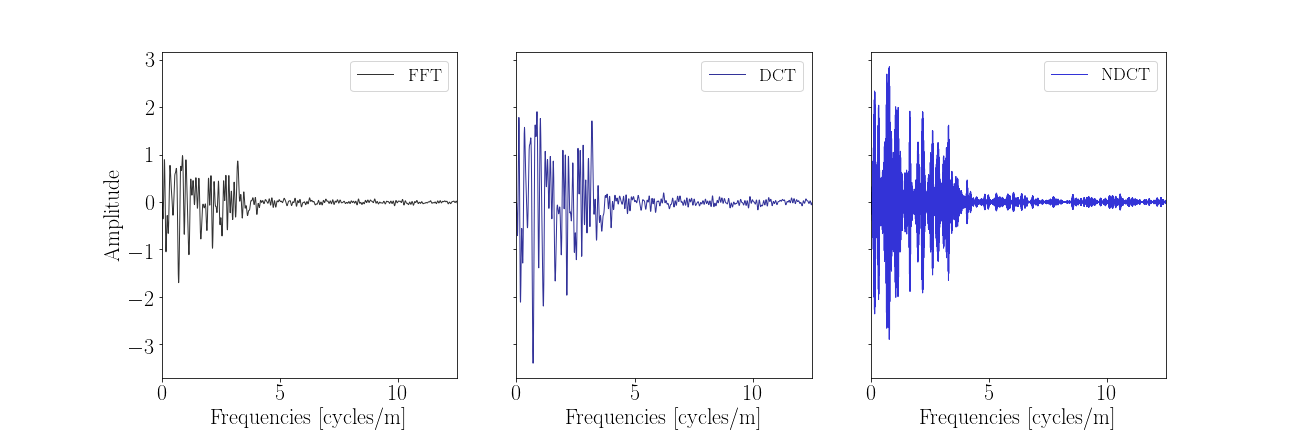
\includegraphics[width=\textwidth]{SpectralTransforms_3.png}
	\caption[FFT, DCT, NDCT, Site A]{\small Examples of three different spectral transforms, FFT, DCT, NDCT, performed on the depth series between Tambora and Laki eruptions from Site A.}
	\label{fig:SpectralTransforms_3}
\end{figure}

\begin{figure}[h]
	\centering
	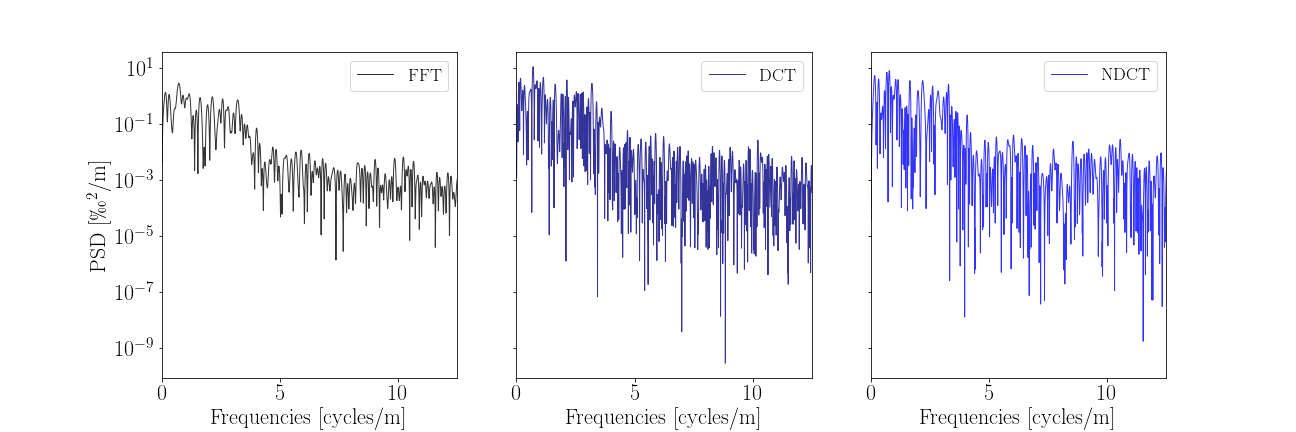
\includegraphics[width=\textwidth]{SpectralTransforms_PSD.png}
	\caption[FFT, DCT, NDCT PSDs, Site A]{\small Examples of power spectral densities related to the three different spectral transforms, FFT, DCT, NDCT, seen in Figure \ref{fig:SpectralTransforms_3}.}
	\label{fig:SpectralTransforms_PSD}
\end{figure}







\subsection[Signal Restoration][Signal Restoration]{Signal Restoration by Optimal Diffusion Length}
\label{Subsec:SignalAnalysis_BackDiffusion_SignalRestoration}
When considering a water isotopic depth series as the ones under examination in this thesis, it is possible to restore some of the signal lost to diffusion. This signal restoration technique will forwardly also be mentioned as 'back-diffusion', as it simulates a process that is the reverse of the diffusion process.

Along with restoring some of the signal, the spectral filtering technique used here also reveals a property of the depth series: an estimate of the diffusion length. This estimate comes from the inherent nature of the noise in the spectrum.

\subsubsection[Spectral Filtering][Spectral Filtering]{Spectral Filtering}
\label{Subsubsec:SignalAnalysis_BackDiffusion_SpectralFiltering}


When examining a real-world signal with focus on the frequency domain one will quickly run into the subject of noise. Different signals are prone to different types of noise, and must thus be treated in a fitting manner. Some spectra are prone to random low frequency noise and some to high, while others again might have a well-defined noise spectrum inherently. Understanding the nature of the noise is crucial for further signal analysis, as the signal-to-noise ratio (SNR) needs to be sufficiently high to be able to accurately separate signal and noise from each other. By understanding the noise, and modelling and estimating it, it can become possible to generate a filter which might minimize the noise and enhance the signal. This next section will go into detail with how to construct a filter fitting to the data at hand. This filtering will also be able to give an estimate of the diffusion length at a given depth section, due to the inherent nature of the signal and noise.

%
%\subsubsection{Kernel Estimation}
%\label{Subsubsec:SignalAnalysis_BackDiffusion_SignalRestoration_KernelEstimation}

Through spectral analysis it is possible to treat the noise of the signal consistently. The goal is to create spectral filters which enhances the signal while minimizing the effect of the noise, thus increasing the SNR.\\
Theoretically, without any diffusion, the change in isotopic concentration would be described through a step function, going from one constant concentration to another. This step function can be described by the Heaviside function:
\begin{equation}
	D(t) = \begin{cases}
		0, & t < 0 \\
		1, & t \geq
	\end{cases}
\end{equation}

In reality, a number of different mixing processes change this step function, and the measured signal will be a smooth curve, $s(t)$, which corresponds to the convolution of $S(t)$ with the mixing response function $M(\tau)$
\begin{equation}
	d(t) = \int_{- \infty}^{\infty} D(\tau) \cdot M(t - \tau)d\tau
\end{equation}

As is well known, in the spectral domain, convolution is multiplication and the mixing is described as the multiplication between the Fourier transform of $S$ and $M$:
\begin{equation}
	\tilde{d} = \tilde{D} \cdot \tilde{M}
\end{equation}


By differentiation with respect to time, the mixing filter $M$ is unaffected, and differentiation of the measured system response, the Heaviside function, $S'$ is a delta function, which Fourier transformed is unity, leading to:
\begin{equation}
	\tilde{d'} = \tilde{D'} \cdot \tilde{M} = \tilde{M}
\end{equation}

The mixing filter can thus be determined by measuring the system response to a step function, differentiating performing Fourier transform of the result $d'$.

After determination of the mixing filter $\tilde{M}$, the unmixed signal $D$ can be estimated in theory by inverse Fourier transform of


\begin{equation}
	\tilde{D} = \tilde{d}\cdot\tilde{M}^{-1}
	\label{eq:Restoration}
\end{equation}

During the mixing, cycles with short wavelengths are heavily washed out, and through the restoration in Eq. \ref{eq:Restoration}, the amplitudes corresponding to these wavelengths are heavily amplified by the filter. This method though has a drawback, which is that when the measurements contain noise, the restored signal will be dominated by high-frequency noise, greatly amplified by the mixing filter. Thus it is a problem of retaining as much (short wavelength) signal as possible while simultaneously attempting to amplify the high-frequency noise as little as possible. This optimal trade-off can be found by creating an optimum filter for the considered measured isotopic signal:
\begin{equation}
	\delta_M(z) = \delta_m (z) + \eta(z)
\end{equation} 

This optimal (Wiener) filter $\tilde{F}$, defined for each wave number $k = 2\pi \omega$, is presented as the ratio between pure signal and pure signal plus noise described in Power Spectral Densities as:
\begin{equation}
	\tilde{F}(k) =\frac{|\tilde{\delta_m}(\omega)|^2}{|\tilde{\delta_m}(\omega)|^2 + |\tilde{\eta}(\omega)|^2}
	\label{eq:WienerFilter}
\end{equation}

In this work, the power spectral densities of the signal and the noise, respectively, are determined through analysis of the power spectral density of the combined signal/noise PSD.\\
The PSD of the noise free measured signal, $|\tilde{\delta_m}(\omega)|^2$, is assumed describe as 
\begin{equation}
	|\tilde{\delta}_m(\omega)|^2 = P_0 e^{-k^2 \sigma_{\text{tot}}^2}
	\label{eq:SignalPSD}
\end{equation}

where $\sigma_{\text{tot}}^2$ describes the total estimated diffusion length of the mixing.\\
The noise is assumed to be red noise, described by an autoregressive process of first order, AR1:
\begin{equation}
	|\tilde{\eta}(\omega)|^2 = \frac{\sigma_{\eta}^2 \Delta z}{|1 + a_1 \exp(-2\pi i \omega \Delta z)|^2}
	\label{eq:NoisePSD}
\end{equation}
where $\sigma_{\eta}^2$ is the variance of the red noise, $a_1$ is the AR1 coefficient and $\Delta z$ is the resolution of the time/depth data.
It is then possible to estimate the parameters $P_0$, $\sigma_{\text{tot}}^2$, $\sigma_{\eta}^2$ and $a_1$ by curve fitting, separately, the two expressions in Eq. \ref{eq:SignalPSD} and \ref{eq:NoisePSD} to the data. The estimated parameters are varied to find the optimal guess to use for the filter.

\begin{figure}
	\centering
	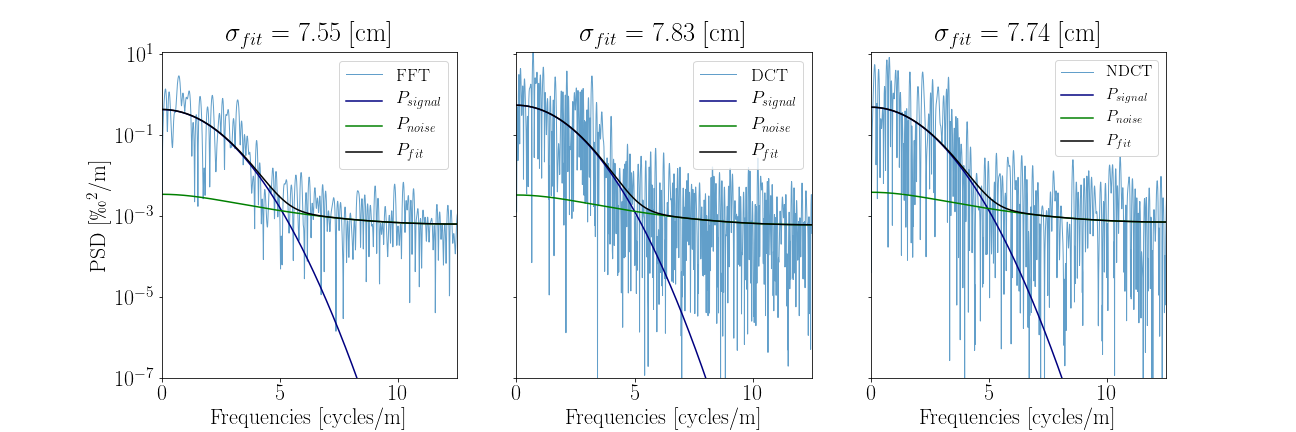
\includegraphics[width=\textwidth]{SpectralTransforms_PSDwFits.png}
	\caption[FFT, DCT, NDCT PSDs with Fit, Site A]{\small Noise, signal and total fit to PSD, illustrating the construction of the Wiener Filter, see Sec. \ref{Sec:SignalAnalysis_Restoration}.}
	\label{fig:SpectralTransforms_PSDwFits}
\end{figure}

An example of the constructed Wiener filter can be seen in Figure \ref{fig:SiteA_WienerFilters} on both a linear and a double logarithmic scale.


\begin{marginfigure}
	\centering
	\begin{subfigure}{\marginparwidth}
		\centering
		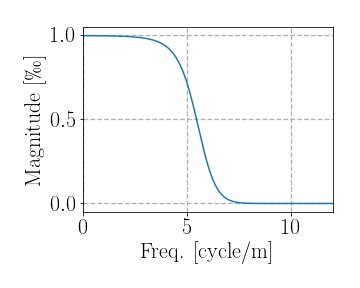
\includegraphics[width=\textwidth]{SiteA_WienerFilter.jpg}
		\caption{\footnotesize}
		\label{fig:SiteA_WienerFilter}
	\end{subfigure}\\[1ex]
	
	\begin{subfigure}{\marginparwidth}
		\centering
		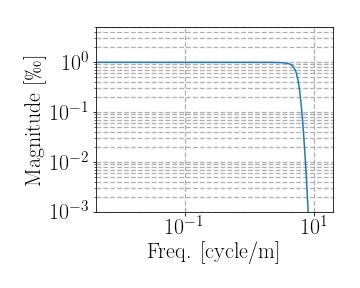
\includegraphics[width=\textwidth]{SiteA_WienerFilter_loglog.jpg}
		\caption{\footnotesize}
		\label{fig:SiteA_WienerFilter_loglog}
	\end{subfigure}
	\caption[Wiener filter]{\footnotesize\textbf{(a)} Wiener filter on linear scale. \textbf{(b)} Wiener filter on double logarithmic scale.}
	\label{fig:SiteA_WienerFilters}
\end{marginfigure}

\subsubsection[Final Restoration][Final Restoration]{Final Restoration}
\label{Subsubsec:SignalAnalysis_BackDiffusion_FinalRestoration}

After finding the best fit (noise and signal) to the spectral data, it is possible to construct an optimal restoration filter, $\tilde{R}$, which contains two separate filters. The one is the Wiener filter, $\tilde{F}$, which is described in the above section and the other is a Gaussian filter constructed to amplify certain frequencies [REFERENCE]. This filter, the transfer function of the system, is constructed to specifically amplify the frequencies heavily attenuated by the diffusion process and is described as
\begin{equation}
	\mathcal{G} = \frac{1}{\sigma\sqrt{2\pi}} e^{\frac{-z^2}{2\sigma^2}},
	\label{Eq:TransferFct_z}
\end{equation}

in the time(depth) domain and, since the Fourier transform of a Gauss is still a Gauss, in the frequency domain it is described as:

\begin{equation}
	\tilde{\mathcal{G}} = \mathcal{F}[\mathcal{G(z)}] = e^{\frac{-(2\pi\, f)^2\sigma^2}{2}}.
	\label{Eq:TransferFct_frq}
\end{equation}

Finally, the constructed frequency restoration filter, in the frequency domain, is a product of the Wiener filter, from Eq. \ref{eq:WienerFilter}, and the transfer function, from Eq. \ref{Eq:TransferFct_frq}:

\begin{equation}
	\tilde{R} =  \tilde{F} \cdot \tilde{\mathcal{G}}^{-1}
\end{equation}
which results in a rewrite of equation \ref{eq:Restoration} to:
\begin{equation}
	\tilde{D} = \tilde{d}\cdot\tilde{F}\cdot\tilde{\mathcal{G}}^{-1}
\end{equation}

An example of the final frequency restoration filter, as it changes with diffusion length estimate inputted in the transfer function, $\tilde{\mathcal{G}}$, can be seen in Figure \ref{fig:SiteA_filtersEx}.

\begin{figure}[h]
	\centering
	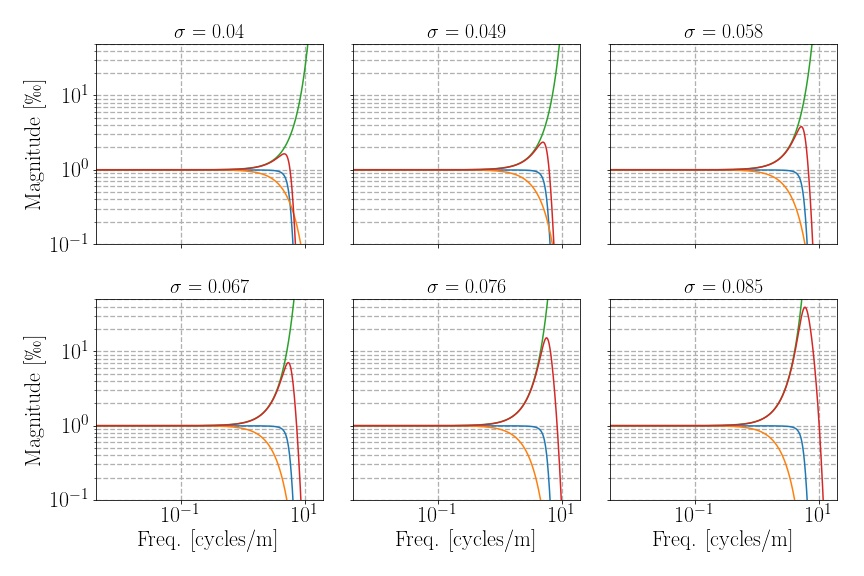
\includegraphics[width=\textwidth]{SiteA_filtersEx.jpg}
	\caption[Frequency filters example, Site A]{Frequency filter examples ranging from diffusion length 0.04 m to 0.085 m.}
	\label{fig:SiteA_filtersEx}
\end{figure}


\subsection[ALT from Spectral Analysis]{Annual Layer Thickness Estimates}
\label{Subsubsec:SignalAnalysis_SpectralAnalysis_ALT}

The transfer function of the diffusion process, Eq. \ref{Eq:TransferFct_frq}, can be rewritten as a function of the wavelength of the isotopic signal, $\lambda$:
\begin{equation}
	\tilde{\mathcal{G}} = e^{\frac{-2\pi^2\sigma^2}{\lambda^2}}
	\label{Eq:TransferFct_lambda}
\end{equation}

The wavelength of the signal corresponds roughly to the annual layer thickness(ALT), $\lambda_A$, in the signal. Regarding the isotopic signal as a wave, it is clear from both theoretical knowledge of the processes and visual inspection of the data, that the diffusion and densification have an effect on the magnitude and the wavelength/frequency respectively. The diffusion attenuates some of the waves magnitude, and the densification shortens the wavelength of the signal. Since both magnitude and wavelength are aspects of a wave, the general effects of the densification and diffusion processes can be examined by spectral analyzing the entire core. This is done by dividing the signal into a number of sections of an (almost) fixed length, $l_{sec}$ and shifting this section down through the core with a shift of length $l_{shift}$. The length is not exactly fixed, as the sample sizes vary through the core, which results in small variations in section and shift lengths.

From the spectral analysis, an estimate on the annual layer thickness can be given, corresponding to the most prominent frequency peak in the spectrum. Sometimes, though, the most prominent peak might be a resonance frequency at some value below that of the frequency related to the ALT. This has been dealt with in this thesis by simply assuming that the frequency in section $l_{sec}^i$ must be larger than the frequency in $l_{sec}^{i-1}$, and the analysis is then carried out be sequentially going through the depth segments. Since different spectral transforms have already been introduced, it was obvious to compute the spectral analysis and most prominent frequency through more than one spectral transform. Thus DCT, NDCT, FFT and MEM has been used, and the found frequencies have then been used to estimate and average wavelength, and thereby ALT, in the given section, see Figure \ref{Fig:SiteB_0-5m_ALTestimate_example} showing a spectral analysis with 4 different transforms of the first 5 meters of the core drilled at Site B.

\begin{marginfigure}
	\centering
	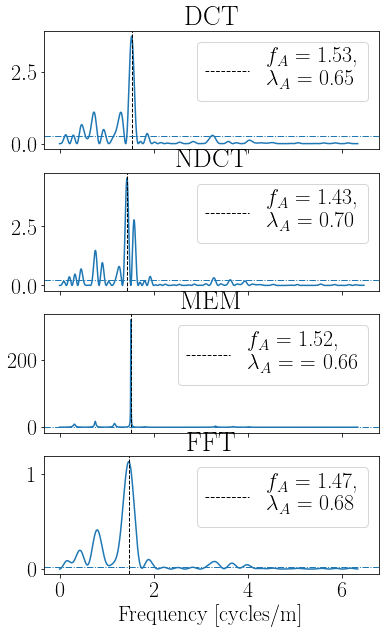
\includegraphics[width=\marginparwidth]{ALTestimate_example.png}
	\caption[]{\small Example of annual layer thickness estimation for section of 5 meters at depth [0;5] m, Site B.}
	\label{Fig:SiteB_0-5m_ALTestimate_example}
\end{marginfigure}

\begin{figure}[h]
	\centering
	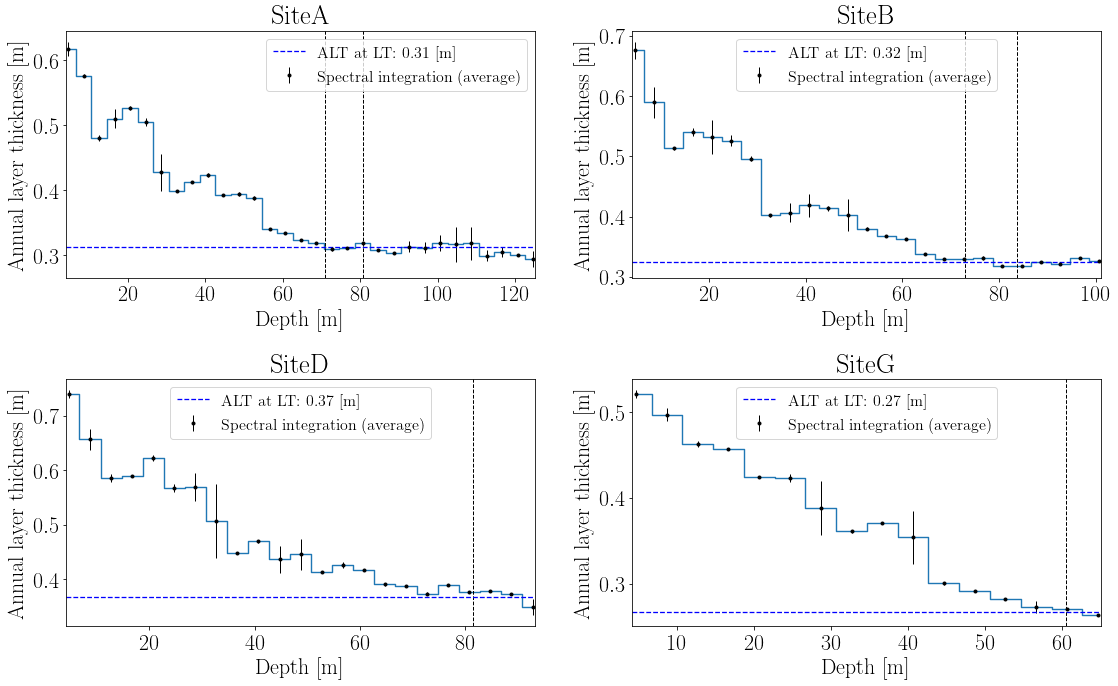
\includegraphics[width=0.95\textwidth]{AllCores_ALT_l5_s4.png}
	\caption[]{\small }
	\label{Fig:AllCores_ALT_l5_s4}
\end{figure}

Figure \ref{Fig:AllCores_ALT_l5_s4} shows the ALT estimates of the entire cores drilled at site A, B, D and G. The section length is 5 m and the shift is 4 m, to avoid missing any frequencies in the transitions between sections. Along with the estimated ALTs, an estimate of the average ALT value at the depth corresponding to between Laki and Tambora events has also been shown. 

In the method section in the following chapter, the stability of this method is tested, and the optimal parameters for $l_{sec}$ and $l_{shift}$ are estimated.


\section[Peak Detection]{Peak Detection}
\label{Sec:CompMeths_PeakDetection}

Knowing that water isotopic data are a proxy for temperature, the most obvious way to determine annual layers in the signals is by detecting peaks and troughs. During colder periods, e.g. winter, the air masses arriving at the ice core sites have formed more precipitation before reaching the sites, and the vapor that results in this final precipitation is then more depleted of heavy isotopes, resulting in lower isotopic values, troughs in Figure \ref{Fig:ICE_Crete_10m_dated}. The precipitation falling during warmer conditions, e.g. summer, is correspondingly less depleted of the heavy isotopes, and results in higher isotopic values, peaks in Figure \ref{Fig:COMPMETH_Crete_10m_PeaksTroughs}.
\begin{figure}[h]
	\centering
	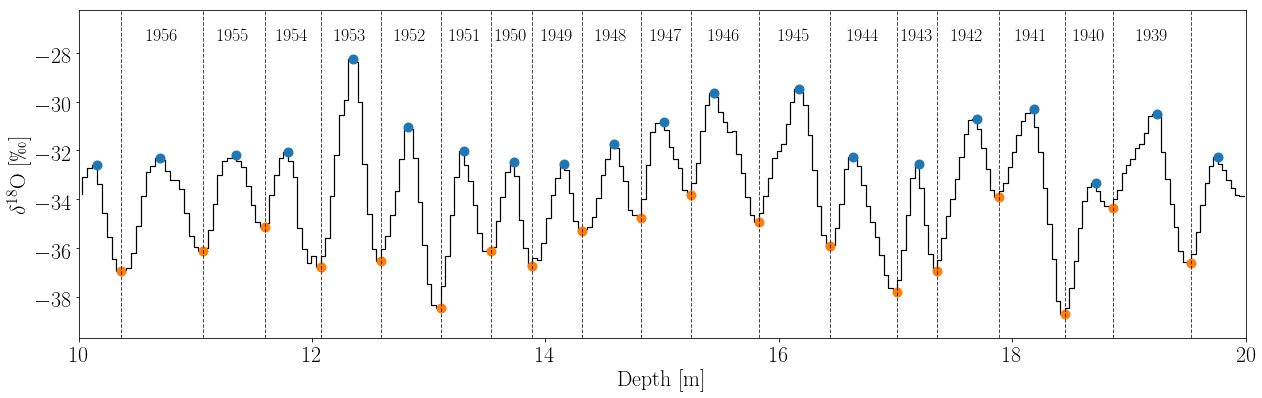
\includegraphics[width=\textwidth]{Crete_10m_PeaksTroughs.png}
	\caption{\small Ten meters of the top of Cretê ice core, with identification and dating of 19 annual layers, with peaks(blue) corresponding to summers and troughs(orange) corresponding to winters.}
	\label{Fig:COMPMETH_Crete_10m_PeaksTroughs}
\end{figure}

Peak detection and layer counting has previously been carried out by visual inspection of the ice core depth signals, but as computers and algorithms have become more integrated in data analysis, it is now more common to use different computational methods. Developing and implementing layer counting and peak detection algorithms can be done in a number of different ways, but for this project, at first a very simple method has been initially implemented and later the method has been improved and optimized through a number of different constraints. One could also use different pattern recognition techniques[REFERENCE]\todo{References here.} to achieve more intelligent detection, and later some of these methods will be presented.

The most naïve approach, and the one first implemented in this project, to peak detection is to simply find local maxima by comparing neighbouring values. When examining point $d_i$, the point is deemed a local maxima, if $d_{i\pm1} < d_i$. Local minima, troughs, can be found in exactly the same manner by finding minima as $d_{i\pm1} > d_i$. A very simple constraint for this method is to keep a required minimal distance between peaks, so that two peaks cannot be detected within a point distance of $\Delta d_{\text{min}}$. For example at a depth of 12 m in Figure \ref{Fig:COMPMETH_Crete_10m_PeaksTroughs} two troughs can be seen, but only one is chosen, as they are within the threshold distance to each other, which here is set to $\Delta d_{\text{min}} = 7$ points. Here, the lowest of the two troughs is chosen. The threshold distance can be chosen in different ways, for this short section it has been chosen through visual inspection, but more generally it can be chosen by examining some of the intrinsic properties of the signal, more about this in Section \ref{}.

\todo{COMPMETH-PEAKDET: Write about better peak detection with cubic spline interpolation (enhanced resolution)}

\subsection[Constrained Peak Detection]{Constrained Peak Detection}
\label{Subsec:CompMeths_PeakDetection_Constrained}
For better peak detection, a number of constraints have been implemented. Mainly the prominence of the peaks and the distance between neighbouring peaks have been considered. These parameters are examined, since it is possible to make a qualified estimate on the minimum distance between neighbouring peaks through the ALT estimation described above, and on the prominence through the amplitude attenuation estimates. 



\subsubsection[Optimal Choices]{Optimal Parameter Choices}




\section[Splines and Interpolation]{Splines and Interpolation}	
\label{Sec:CompMeths_SplinesAndInterpolation}
For the purpose of this thesis, interpolation of data needs to be fast, efficient and result in a function as smooth as possible. The last criterion is due to the knowledge of the nature of the data. The measurements are not continuous but should indeed in theory be so. Thus a good choice for interpolation of the data examined in this thesis would be the cubic spline interpolation. An instance of a such interpolation can be seen in Figure \ref{fig:Interp}.

Cubic spline interpolation has been used in two instances during this analysis, both times through the \lstinline[language=Python]|Python SciPy| package \lstinline[language=Python]|scipy.interpolate.CubicSpline|\todo{SIGNAL-INTERP: REFERENCE!!}. Firstly, to assure equally spaced data points, so as to be able to perform a useful frequency analysis through spectral transformation, see Section, \ref{sec:???}. Secondly cubic spline interpolation was used to improve on peak detection in the final back diffused data. The final data have a rather low resolution, leading to an initial guess of peak positioning that might be shifted due to the discretization. Through cubic spline interpolation it is possible to construct a smooth estimate of a signal of higher resolution, leading to a peak positioning estimate that might be less shifted, see Figure \ref{fig:InterpFinal}.


\subsection[Interpolation][Interpolation]{Interpolation}
\label{Subsec:CompMeths_SplinesAndInterpolation_Interpolation}

Interpolation is a tool that can be used - and misused - to extract more information out of a given set of data. Used correctly, interpolation can reveal more information than is initially available and disclose connections not apparent at first, but used incorrectly, it can be manipulated to infer misleading correlations and lead to inaccurate conclusions. Thus it is a tool that must be used with care. Aiming to avoid incorrect deductions and inferences one should at first gain as much knowledge about the data at hand as possible. By understanding how the data have come about and gaining knowledge about the underlying physical theories a somewhat deficient data set can robustly and securely be interpolated to accommodate the needs of the analysis. In the case of this thesis, both knowledge about data gathering and the physics at play have been gained and thus some of the common fallacies may be avoided. The limits of the data available is due to the discrete sampling, leading to a minimum sampling of about 26 samples per meter of ice.
When considering that the depth series of 32 years between Tambora and Laki is just above 10 meters, this means that each meter of ice needs to contain at least three years on average. 26 samples per three years might not sound as a bad sampling interval, but if the goal is to show seasonality and give a best estimate of annual layer thickness, interpolation could be put to good use to be able to give better estimates of the exact placement of peaks and valleys.



\subsubsection[Basic Idea][Basic Idea]{Basic Idea}
\label{Subsubsec:CompMeths_SplinesAndInterpolation_Interpolation_BasicIdea}
\todo{Write short introduction to interpolation here. Reference Appendix.}

\subsection[Interpolation in this Project][Interpolation in this Project]{Cubic Spline Interpolation in this Project}
\label{Subsec:CompMeths_SplinesAndInterpolation_InterpolationInThisProj}
For this project cubic spline interpolation has been implemented and examined in two particular sections of the analysis: 
\begin{enumerate}
	\item Cubic spline interpolation of raw, uneven data to represent even data, that can be analyzed through fast spectral transforms.
	\item Cubic spline interpolation of the final back-diffused signal estimate to enhance resolution for more efficient peak detection.
\end{enumerate}

\subsubsection[Interpolation 1]{Interpolation of Data Before Deconvolution}
\label{Subsubsec:CompMethod_StabilityTests_Interpolation1}

The first interpolation is needed, if the fast spectral transforms FFT or FCT are used, as one of the conditions of the algorithms is that the data are evenly spaced. At first, this was implemented in the analysis, but this had the risk of excluding some information that might lie in the unevenly sampled data. Later, the method was abandoned in favor of implementing a nonuniform spectral transform (NUFT or NDCT), which is slower than the FFT and FCT, but carries all information from the unevenly sampled signal into the spectral domain. Luckily, this nonuniform transform needs only be carried out once, as the inverse transform, i.e. resampling in time domain, can be done uniformly without loss of information and any future spectral transforms can then be performed through FFT or FCT.

Even though the first interpolation method was later abandoned, some analysis was carried out with it to examine the effect of the size of the resampled, interpolated data on the final diffusion length estimate. Examples of a resampled signal can be seen in Figure \ref{Fig:COMPMETH_SiteA_DataSplineInterp} and Figure \ref{Fig:COMPMETH_SiteA_MultiSplineInterp}. Figure \ref{Fig:COMPMETH_SiteA_MultiSplineInterp} shows how sample resolution affects information from the signal. The higher sampling resolution, the more information is retained. But higher sampling resolution also means more data to be analyzed, which might slow down any analysis algorithms developed. This might create some headache if an entire ice core length of a couple thousand meters should be examined, but for this study only af few meters are of interest, and thus it should not create delays in the computation time.

\begin{figure}[h]
	\centering
	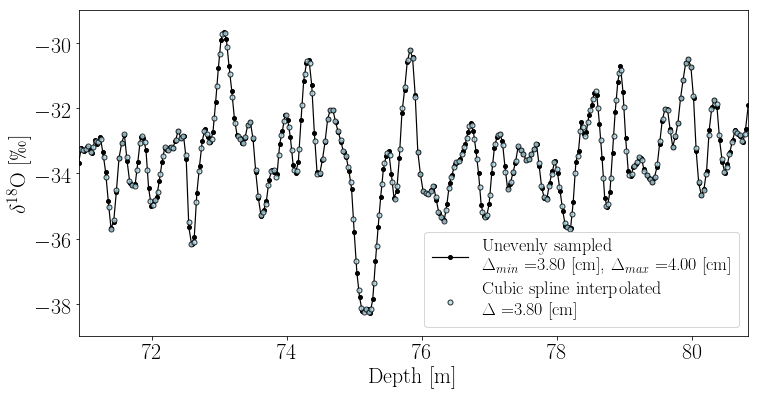
\includegraphics[width=\textwidth]{SiteA_DataSplineInterp.png}
	\caption{\small Unevenly sampled signal from Site A resampled using cubic spline interpolation to an even signal with a new sample size equal to the minimum sample size found in the raw signal.}
	\label{Fig:COMPMETH_SiteA_DataSplineInterp}
\end{figure}

\begin{figure}[h]
	\centering
	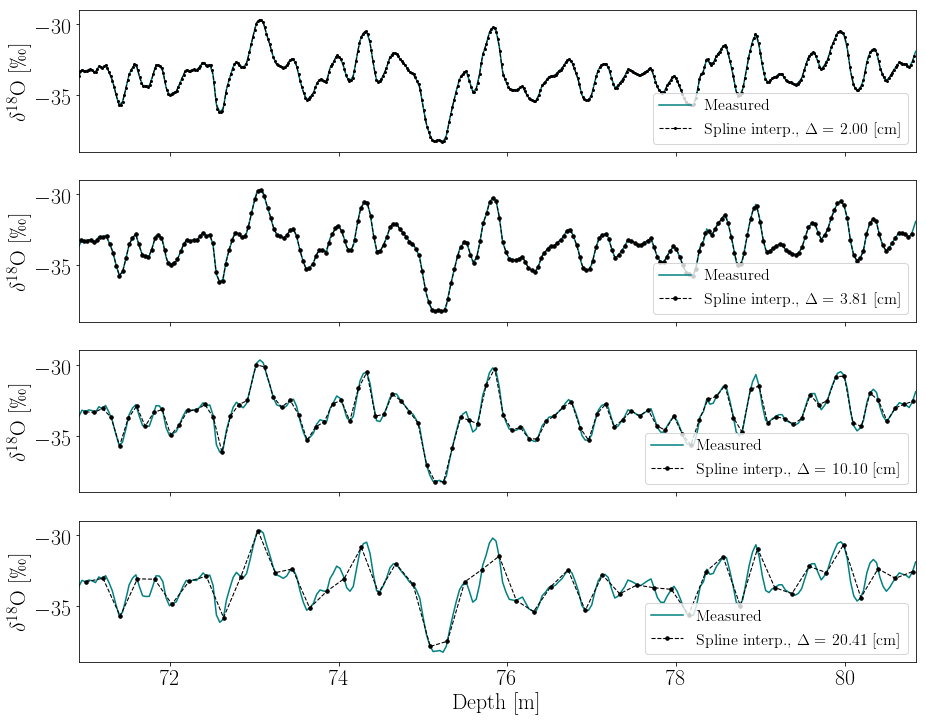
\includegraphics[width=\textwidth]{SiteA_MultiSplineInterp.png}
	\caption{\small Four different resampled signals of Site A data, showing loss of information when resampling resolution is low.}
	\label{Fig:COMPMETH_SiteA_MultiSplineInterp}
\end{figure}

To examine the effect of the resampling resolution on the final diffusion length estimate when conducting a spline interpolation before carrying out the back-diffusion, the full diffusion length analysis has been performed with 100 new interpolation resampling sizes in the range $[\Delta_{\text{min}};\Delta_{\text{max}}]$. This gives an idea of the stability of the method considering both sample size of the raw data and resampling by interpolation. The minimum and maximum interpolation samplings are presented in Table \ref{tab:InterpSamples} and an illustration of the test results can be seen in Figure \ref{Fig:COMPMETH_SamplingVsDiffLen_interpBF}.

\marginnote{%
	\footnotesize
	\centering
	\begin{tabular}{lccc}
		\toprule
		\textbf{Site} & $\Delta_{\text{min}}$& $\Delta_{\text{max}}$ & $\Delta_{\text{OG}}$\\
		& [cm] & [cm] & [cm] \\
		\midrule
		Site A & 1.0 & 10.6 & 3.8-4.0\\
		Site B & 1.0 & 11.7 & 3.8-4.0\\
		Site D & 1.0 & 12.0 & 3.7-3.9\\
		Site E & 1.0 & 11.4 & 4.1-4.4\\
		Site G & 1.0 & 10.3 & 4.0-4.2\\
		\bottomrule
	\end{tabular}
	\captionof{table}{\footnotesize Minimal and maximal new sample resolution used for testing interpolation before back-diffusion. Each test is run with 100 different new sample resolutions between $\Delta_{\text{min}}$ and $\Delta_{\text{max}}$.}
	\label{tab:InterpSamples}
}[0.5cm]%




\begin{figure}[h]
	\centering
	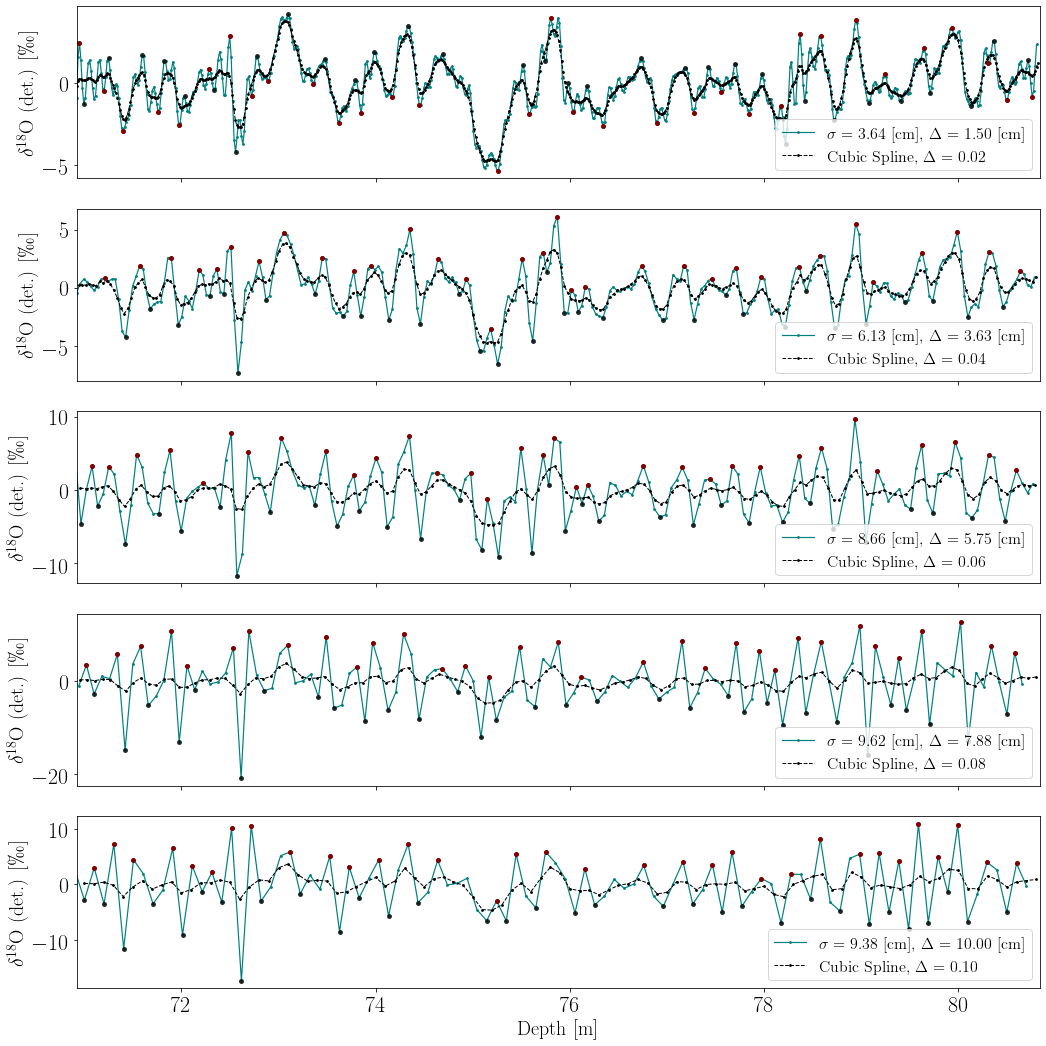
\includegraphics[width=\textwidth]{SiteA_InterpBF_SpecificResamplings.png}
	\caption{\small Site A, illustration of the effect of five different cubic spline resamplings before deconvolution. Original sample sizes lie in the interval [3.80; 4.00] [cm]. Resampling at smaller sample sizes show a tendency to restore some signal frequencies that are not necessarily inherit in the original signal. The resample should thus not be chosen too small as this would introduce some false signal into the results.}
	\label{Fig:COMPMETH_SiteA_interpBF_SpecificSamplings}
\end{figure}

\begin{figure}[h]
	\centering
	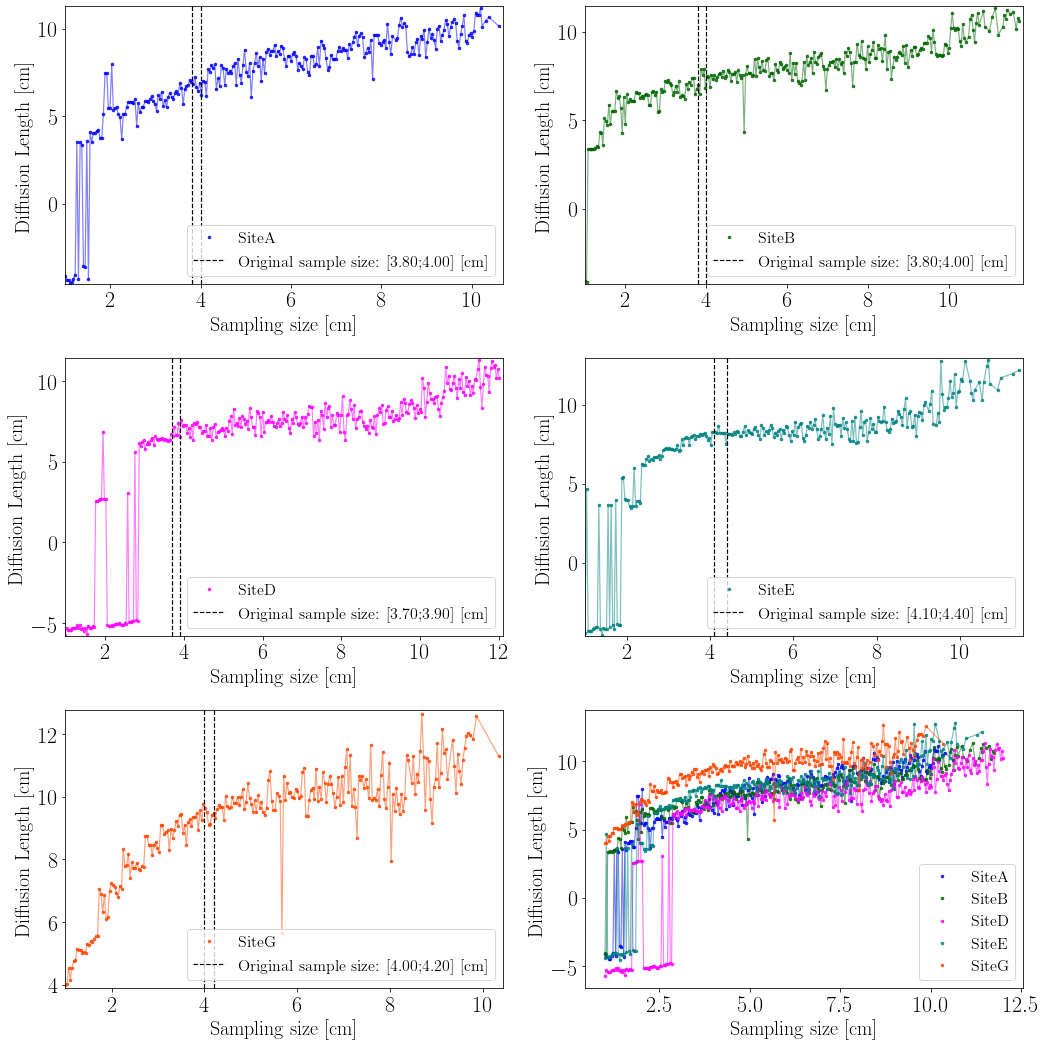
\includegraphics[width=\textwidth]{AllCores_DiffLenVdelta_InterpBF_const.png}
	\caption{\small Diffusion length estimates versus resamples through cubic spline interpolation before deconvolution for Alphabet cores from sites A, B, D, E and G.}
	\label{Fig:COMPMETH_SamplingVsDiffLen_interpBF}
\end{figure}



\subsubsection[Interpolation 2]{Interpolation of Data After Deconvolution}
\label{Subsubsec:CompMethod_StabilityTests_Interpolation2}

The second interpolation is carried out after deconvoluting and back-diffusing the signal, but before detecting peaks. Splines are especially effective when trying to find features like peaks in data which underlying signal is continuous, smooth and differentiable, but the sampling is discrete and thus the data are discrete and non-smooth. The isotopic signal under examination here is assumed to be truly smooth and continuous throughout the core - unless any gaps are present. Thus the cubic spline interpolation is a good tool for estimating a higher resolution version of the final back-diffused data series to use for peak detection. This makes the detection of peaks and troughs more precise, as there might not be a discrete data point exactly at the top of a peak, but the spline interpolation then estimates where the most likely top of the peak must be, on the basis of the existing data. Examples of three different interpolation samplings are presented in Figure \ref{Fig:COMPMETH_SiteA_InterpAF_4samplings}. The effect of resampling after deconvolution on the final diffusion length estimate is illustrated in Figure \ref{Fig:COMPMETH_SamlingVsDiffLen}.

\begin{figure}[h]
	\centering
	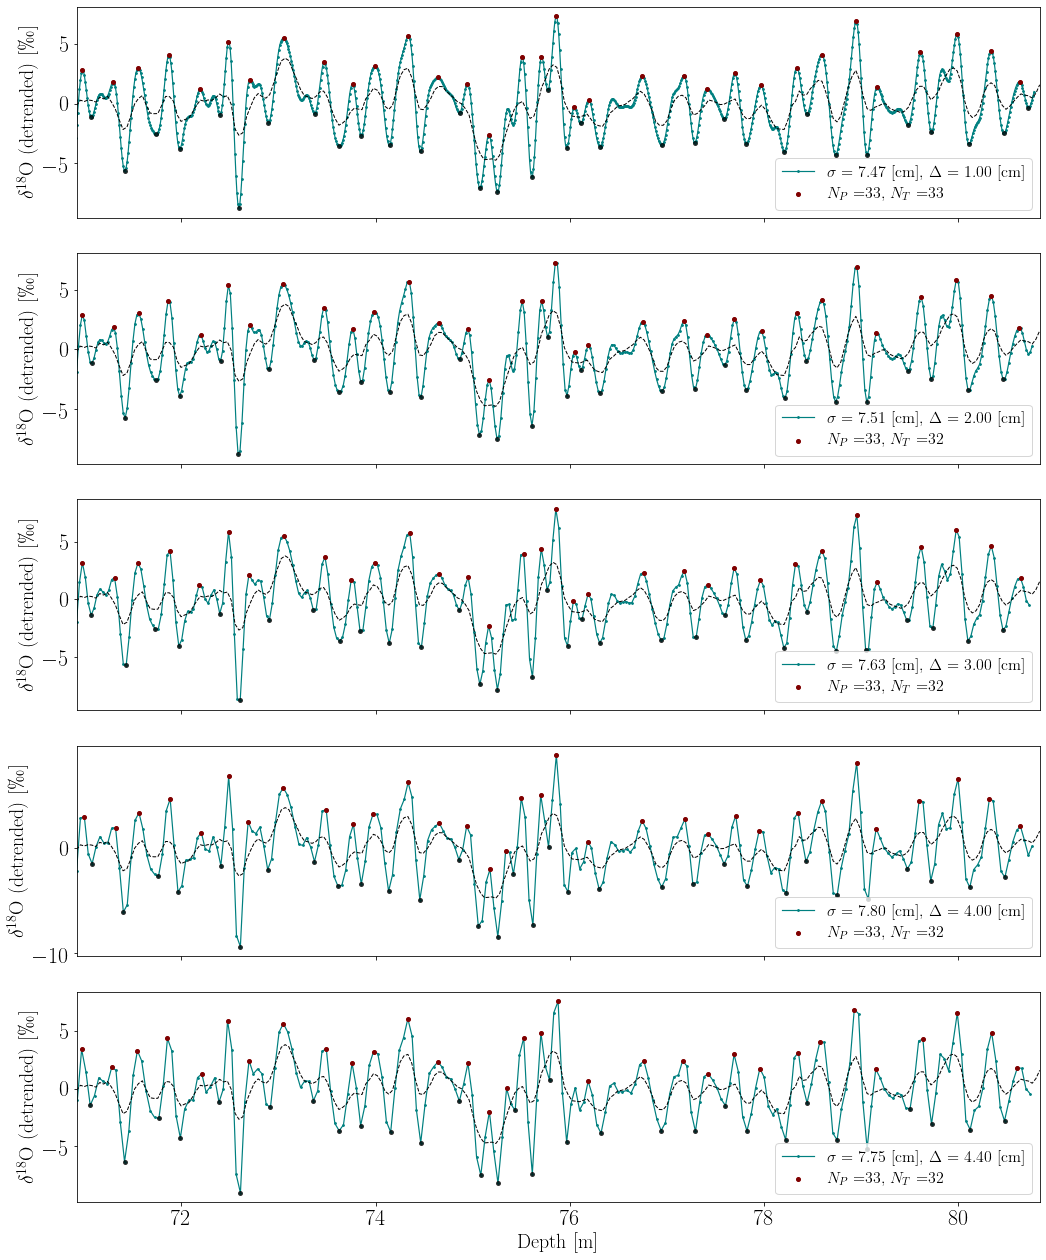
\includegraphics[width=\textwidth]{SiteA_InterpAF_SpecificResampling_BD.png}
	\caption{\small Site A, effect of cubic spline interpolation after signal has been deconvoluted. The interpolation is introduced to make peak detection more stable.}
	\label{Fig:COMPMETH_SiteA_InterpAF_4samplings}
\end{figure}

\begin{figure}[h]
	\centering
	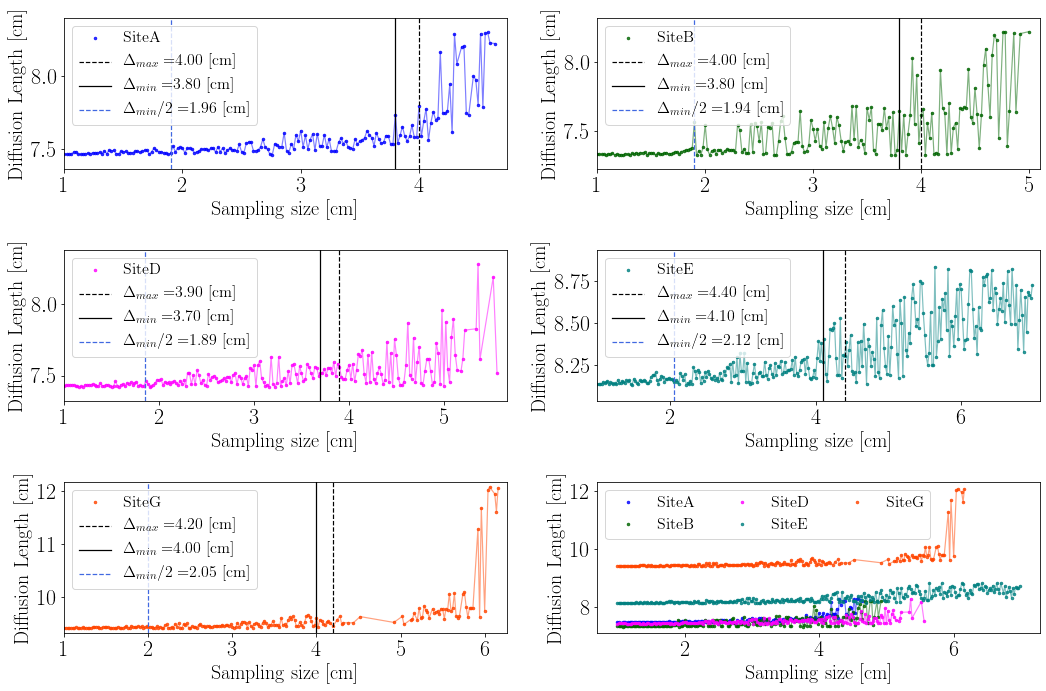
\includegraphics[width=\textwidth]{AllCores_InterpAF_deltaVSdiffLen_BD.png}
	\caption{\small Final diffusion length estimate, given new resample by cubic spline interpolation after deconvolution for Alphabet cores from sites A, B, D, E and G.. The original sample size interval is illustrated as black vertical lines.}
	\label{Fig:COMPMETH_AllCores_SamplingVsDiffLen}\textit{}
\end{figure}









\end{document}
